\documentclass[a4paper,12pt]{article}
\usepackage[margin=1in]{geometry}
\usepackage{enumitem}
\usepackage{amsmath}
\usepackage{mathtools}
\usepackage{amssymb}
\usepackage{graphicx}
\usepackage{placeins}
\usepackage{listings}
\usepackage{tkz-graph}
\usepackage{lipsum}
\GraphInit[vstyle = Shade]
\tikzset{
  LabelStyle/.style = { rectangle, rounded corners, draw,
                        minimum width = 2em,
                        text = red, font = \bfseries },
  VertexStyle/.append style = { inner sep=5pt,
                                font = \Large\bfseries},
  EdgeStyle/.append style = {->, bend left} }
\usepackage{xcolor}
\lstset{language=Matlab,%
    %basicstyle=\color{red},
    breaklines=true,%
    morekeywords={matlab2tikz},
    keywordstyle=\color{blue},%
    morekeywords=[2]{1}, keywordstyle=[2]{\color{black}},
    identifierstyle=\color{black},%
    stringstyle=\color{mylilas},
    commentstyle=\color{gray},%
    showstringspaces=false,%without this there will be a symbol in the places where there is a space
    numbers=left,%
    numberstyle={\tiny \color{black}},% size of the numbers
    numbersep=9pt, % this defines how far the numbers are from the text
    emph=[1]{for,end,break},emphstyle=[1]\color{red}, %some words to emphasise
    %emph=[2]{word1,word2}, emphstyle=[2]{style},    
}
\usepackage{wrapfig}

\begin{document}


\title{Vector Dynamics Generational Model -- Results}
\author{Emma Davis}
\date{\today}
\maketitle

\section{Results}

Plan:

\begin{itemize}
\item Figure 1: Comparing prevalence against vector control (bednets,IRS,larvicides) efficacy for the ODE and generation model. Three plots, one for each control method, with ODE and generational plotted on each.
\item Figure 2: Looking at how the repelling effect of bednets changes feeding cycle length $\rightarrow$ this will also impact incubation period
\item Figure 3: Comparing effect of different vector control measures on vector population size.
\item Figure 4: Population density plots (with SEI), a fixed mid-case for each of: no control, bednets, IRS, larvicides. Show change in population size as well as generational density -- scale.
\item Relationship between force of infection on hosts and probability of a mosquito getting infected (look at different bednet coverages).
\item Comparison of $R_0$ etc for different vector control settings.
\item Use $N_i$ to work out how many infectious vectors will go on to bite at least once more (immediately post end of latent period?). Average number of bites an infectious vector will make?
\item Comparison with Imperial model -- what are the differences we see in the results?
\end{itemize}

\noindent Summary of all results so far: All figures -- add/remove as necessary. Make sure to link back to intro/methods and the structure of the model as well as the implications.\\

\begin{figure}[h]$
\begin{array}{cc}
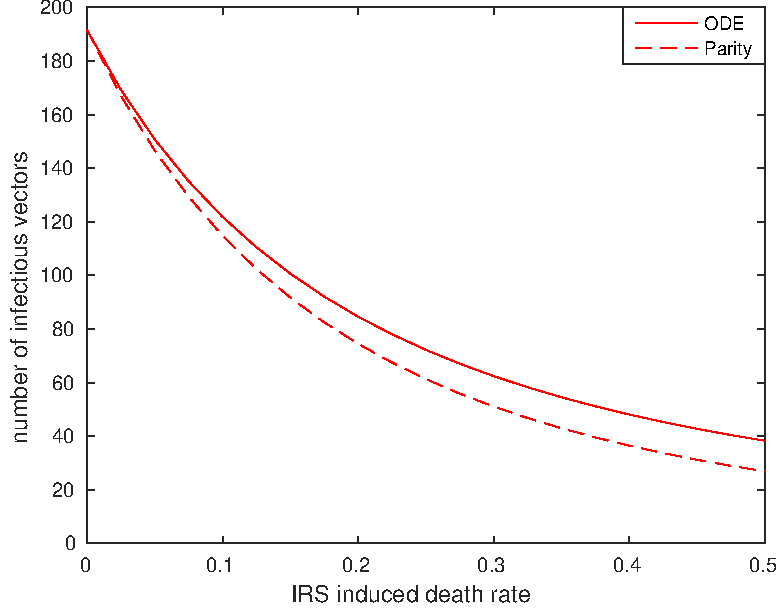
\includegraphics[height=6cm]{modelcomparison_bednets_zeros.pdf}&
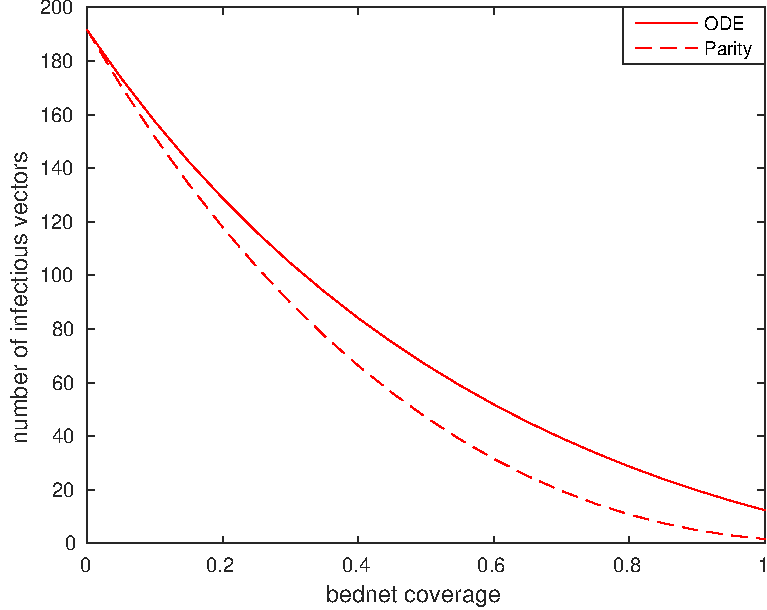
\includegraphics[height=6cm]{modelcomparison_IRS_zeros.pdf}\\
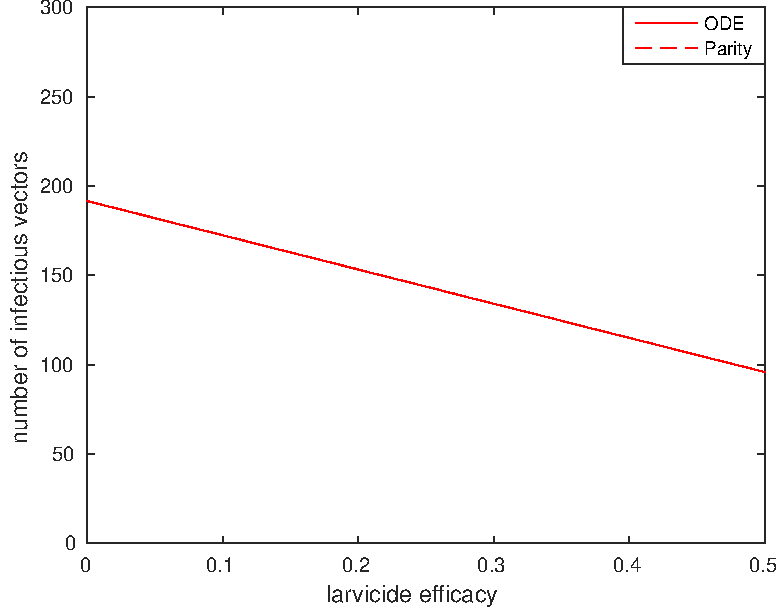
\includegraphics[height=6cm]{modelcomparison_larvicides_zeros.pdf}
\end{array}$
\caption{Plots comparing infectious vector counts for the ODE model and the Parity-based distribution model. Incubation period = 3 generations, birth rate = 500 per day.}
\label{fig:modelcomp}
\end{figure}

\begin{figure}[h]$
\begin{array}{cc}
\includegraphics[height=6cm]{gonocycle_change.pdf}&
\includegraphics[height=6cm]{gonocycle_days.pdf}\\
\includegraphics[height=6cm]{incubationperiods_bednets.pdf}
\end{array}$
\caption{Plots showing the repelling effect of bednets on cycle length due to repeating before feeding.}
\label{fig:incub}
\end{figure}

\begin{figure}[h]
\includegraphics[height=6cm]{PopSizeVCcomp.pdf}
\caption{Plot showing how the population size changes with scale-up of vector control measures: bednets (blue), IRS (--), larvicides (-.-).}
\label{fig:popsize}
\end{figure}

\begin{figure}[h]
\includegraphics[height=11cm]{ComparingControls.png}
\caption{Plots showing the number of vectors in the emerged state of each generation at equilibrium, given by the generational model. Bednet coverage, $\omega=0.45$; additional death rate causes by IRS, $\gamma=0.15$; reduction in birth rate, $\lambda=0.25$. Control measure levels chosen to represent mid-range scenarios and give a similar reduction in total population size (see Table \ref{table:midcases} for exact numbers). Incubation period = 3 generations.}
\label{fig:midcases}
\end{figure}

\begin{table*}[t]
\caption{Population and epidemiological results for the vector control scenarios given in Figure \ref{fig:midcases}. All values given relate to the emerged population only.}% title of Table
\vspace{.1cm}
\centering % used for centering table
\begin{tabular}{|c| c c c c|}% centered columns (5 columns) 
\hline                    %inserts horizontal line
 &  & Control & method  & \\

 & None & Bednets & IRS & Larvicides \\ [0.5ex]% inserts table 
%heading
\hline
Pop size, $N$ & 554 & 411 & 406 & 416\\
\hline                  % inserts single horizontal line
Prevalence & 0.325 & 0.129 & 0.212 & 0.325 \\% inserting body of the table
\hline
Relative $N_I$ & 1.00 & 0.293 & 0.478 & 0.750 \\
[1ex]      % [1ex] adds vertical space
\hline%inserts single line
\end{tabular}
\label{table:midcases}% is used to refer this table in the text
\end{table*}

Notes about Figure \ref{fig:midcases} and Table \ref{table:midcases}
\begin{itemize}
\item Bednets slow down feeding $\rightarrow$ see an increase in number of vectors in early generations (0 and 1).
\item Bednets and IRS both increase the death rate $\rightarrow$ the numbers in each generation drop off quicker.
\item Larvicides reduce each generation by $\lambda$\%, so force of infection will be lowered, but prevalence is unaffected.
\item Peaks in exposeds and infecteds are less pronounced in the presence of bednets $\rightarrow$ this will be caused by the increase in length of the average feeding cycle.
\item Bednets give the largest decrease in prevalence and relative numbers of infecteds, when compared to the other control methods, for an equivalent vector population size.
\end{itemize}

%\bibliographystyle{elsarticle-harv}
\bibliographystyle{unsrt}
\bibliography{report}

\end{document}

%%
%% End of file `ejemplo latex RIAI.tex'.